
\section{The Phase II Project}
\label{sec:phaseII}
%% {\em Provide an explicit, detailed description of the Phase I research
%%   approach and work to be performed.  Indicate what will be done, by
%%   whom (small business, subcontractors, research institution, or
%%   consultants), where it will be done, and how the work will be
%%   carried out.  If applicant is making a commercial or in-kind
%%   contribution to the project, please describe in detail here.  The
%%   Phase I effort should attempt to determine the technical feasibility
%%   of the proposed concept which, if successful, would provide a firm
%%   basis for the Phase II grant application.

%%   Relate the work plan to the objectives of the proposed project.
%%   Discuss the methods planned to achieve each objective or task
%%   explicitly and in detail.  This section should be a substantial
%%   portion of the total grant application.} 

\subsection{Technical Objectives}
%% {\em State the specific technical objectives of the Phase I effort,
%%   including the questions it will try to answer to determine the
%%   feasibility of the proposed approach.}

The requirements being addressed include the development of a robust framework 
for in-situ verification and validation in general purpose numerical simulation 
packages. In particular, the objective of this project is to address the need
for tools that automate verification of end-user numerical solutions in the 
NEAMS toolkit and workbench. 

In Phase II, RNET Technologies and ORNL will pursue the following objectives:

\begin{enumerate}

\item \rnetprop{Harden and extend the core VnV functionality developed during phase I. In particular, the phase II effort 
will look to determine the optimal approach for implementing the run time configurable test injection system such that 
the risks associated with memory corruption and constant correctness are minimized. This objective will include the miscilanious tasks
required to prepare the framework for release, including integration with a unit testing framework, futher development of the documentation generation 
engine, and documentation. }
\item \rnetprop{Develop mechanisms for efficient data movement in a distributed environment. This objective will 
look to determine and implement optimal approaches for comparing data stored in distributed arrays against an expected 
result stored on disk. The key issue here is to define approaches for describing the domain decomposition of the distributed 
array such that the experimental data can be distributed in an efficient manor. In-situ
comparison of variables with experimental and/or analytical results will be a defining feature of the framework because it significantly 
reduces the amount of IO required in \VV testing, while also providing a fine grained mechanism for detecting at what point a solution diverges from
the expected result.}
\item \rnetprop{Optimize test execution times. Initial development will focus on mechanisms for offloading tests to an external server. Offloading of tests to an
external VnV testing service has the potential to significantly reduce overall runtime. This key issue to address here 
will be to develop a mechanism for offloading data such that the data transfer is faster than simply running the test in-situ. The initial focus will be 
on determining the best framework for offloading simple tests (MRNet, SNOBall, ADIOS streaming, etc.). After that has been implemented, the focus will shift
toward implementing job based parallelism for tests the require the simulation to be run multiple times. }
\item \rnetprop{ Develop a robust set of generic \VV tests. The development of these tests (e.g., mesh refinement studies, the method of manufactured solutions, sensitivity analysis, uncertainty quantification) will further equip the users with the tools required to robustly perform end-user \VV.  The open research question the Phase II project will look to address is the optimal approach to integrating existing implementations of the tools (i.e., NIMROD, DAKOTA, MASA) into the in-situ \VV testing framework. Another open question is the development of a generic interface for mesh refinement studies such that we can automatically generate the required grid hierarchy.}
\item \rnetprop{Demonstrate the value of the VnV framework as a component in the NEAMS tools and into the NEAMS workbench. The true benefit of  
the VnV toolkit will only be realized if we can drive wide scale uptake across the entire numerical simulation community. By showing the toolkit can be used 
in the NEAMS tools, and in particular, MOOSE, libMesh and PETSc, we will demonstrate true potential of the product in libraries that are already considered 
cutting edge across the industry. Integration into the NEAMS tools will answer the NEAMS call for tools that support end-user verification
of numerical simulations. Integration into the NEAMS workbench will provide access to the tools in the seamless manor users of the workbench have come to expect. } 

\end{enumerate}

\subsection{Work Plan}
\label{sec:workplan}

As described in the objectives, the final deliverable of the Phase II project will be a fully functional, effcient, battle tested framework 
for integrating advanced end-user verification and validation into general purpose numerical simulation packages. In what follows, we outline
the work required to satisfy the objectives outlined in the previous section and to acheive these goals. 

\subsubsection{Hardening and Optimization of the Injection Point System}

The injection point system developed during Phase I uses C style Macros and string based (void*) pointer casts to declare the variables available for inspection
at each injection point.  When implemented correctly, this is an efficient (void* casts are almost free) and portable (it uses low level C functionality supported by all C/C++ compilers) approach. In Phase II, the project team will develop a custom compiler that supports an annotation based specification for the injection points and the injection point variables. This annotation based specification will be designed to address two key issues with the Phase I approach:

\begin{itemize}
 \item {\bf String based pointer casts:} The injection point system developed in Phase I requires the developer to provide a string that describes the type for each variable available at an injection point. Under the hood, the injection point system using string comparisons to ensure compatibility been test parameters and injection point variables. The key issue with this approach is that the strings specified at each injection point cannot be verified during compilation.  This will causes major issues in cases where, say, the developer changes the type of a variable, but forgets to update the type string in the injection point. The custom source code processor developed in Phase II will automatically detect the type of the variables passed to the injection point system, removing the requirement for a hard-coded type string. 
  
 \item {\bf Restrictive type specifications:} The current system uses C compliant pre-processor macros to simplify the process of describing injection points and variables. The benefit of this approach is that the injection points can be compiled into any application without significant changes to the build system. The downside is that single-pass, text based macros place a significant restriction on the functionality that can be implemented. The annotation system developed in Phase II will be far more dynamic, allowing users to full control over what variables can be accessed at each injection point, including the ability to provide access to internal components of data structures, describe the domain decomposition of distributed arrays and to complete pre-test processing of variables. The annotation system will also provide a mechanism for suggesting default tests to be run at each injection point, and will provide a mechanism for injection point detection in non-object orientated programming languages where runtime injection point detection cannot be completed.  
\end{itemize}

This compiler will be written using Clang. Clang is a compiler front end for the C family of languages. It is a well supported, well documented compiler package designed as a drop in replacement for GCC. In particular, Clangs simple API for defining custom Pragma routines, combined with its robust API for walking the Abstract syntax tree of the code make it the perfect choice for developing this annotation based system for defining injection points. Clang has seen wide scale uptake across the software development world and, in recent years, has emerged as a realistic competitor to the ubiquitous GCC compiler suite.  

Figure~\ref{TODO} shows how the annotation based injection point system will look in a C/C++ code. The user will annotate simple variables with the ``@Variable(''IP\_1``, ''IP\_2``,...)'' annotation. In that annotation, users will be able to specify the injection points for which that variable is available. Additionally, users will be able to specify additional parameters that define how the variable should be accessed, e,g., for providing access to a member of a struct (line TODO), or for providing access to a certain element in an array (line TODO). For distributed arrays, the annotation based system will allow users to define approaches for obtaining the global and local ownership for each processor. Together, this annotation based system will allow users to fully control the access to these variables. The original Phase I approach will still be available for users that cannot switch to the new Clang compiler. Where possible, the custom compiler will make use of available C++11 RTTI information (dynamic\_cast, typeid, etc.); however, a general C approach will be favored due to the large number of C programs still regularly used in scientific computing. 


\subsubsection{Efficient Statistical Comparisons in Distributed Settings} 

One of the major benefits of the VnV framework is that it allows for in-situ testing and analysis in distributed systems. In particular, this type of in-situ analysis is particularly useful for analyzing and comparing data stored in distributed arrays. For example, a tests could be used to assert that all the elements in an array are positive, or that all the elements in an array are the same as the elements in another array; all without ever writing the data to disk and/or without collecting the data on a head node. 

To that end, the Phase II project will research efficient techniques for analyzing, asserting and comparing data stored in distributed arrays. To achieve this, the project team will need to address two key issues; determining the data decomposition and efficiently performing the statistical analysis. 

{\bf Data decomposition:} In order for the testing algorithms to act of the data structures, some information about the global distribution of the data will be required. Determining this global partition is not difficult for programs that use a regular decomposition scheme because, in these cases, there exists a static mapping function that can be evaluated locally on any processor to determine the owner of any index. For programs using irregular decompositions, no such mapping exists. Instead, for irregular domains, it is necessary to calculate the global partition dynamically at runtime. Hence, a major goal of the Phase II project will be to implement an efficient, scalable approach to dynamically obtaining the global partition from generic distributed arrays. 

To do this, the project team will investigate several approaches to determining intra-processor communication patterns for distributed data. 

The first approach implemented will be to generate the global partition through a collective MPI communication (MPI\_AllGatherV). In this setting, the global partition is assembled on every processor. This makes determining the owner of a particular data component a simple task. 

The above approach requires O(P) storage on each processor and O(log(P)) communication costs (where P is the number of processors). For small processor counts, this linear dependence on P for storage costs is not likely to be a problem. However, in large-scale settings this will quickly become an issue \cite{hypre-assumed}. In particular, such storage costs are an issue for VnV testing because they will be required on top of the storage costs associated with the application being tested. 

To address these storage concerns, the project team will implement an Assumed partition algorithm. This algorithm was first introduced in \cite{} as an efficient mechanism for determining intra-processor communication patterns in Hypre, a scalable collection of high performance linear solvers. The assumed partition algorithm is a parallel rendezvous algorithm that facilitates intra-processor communication using O(1) storage and O(log(P)) communication. The algorithm can be characterized by the following three steps;
\begin{itemize}
 \item Step 1: Assume the global distribution of data 
 \item Step 2: Redistribute the actual partition description to the assumed partition
 \item Step 3: Use the assumed partition to determine global information
\end{itemize}

The key to the assumed partition algorithm is that it assumes the data is distributed using a regular distribution that 
can be queried locally on each processor using a O(1) function call. Step 2 of the algorithm, the data required to form a distributed directory
containing information about the actual data distribution is communicated to the assumed partition. Once this distributed directory has 
been formed, it can be directly queried to determine the owner of the required data in the actual distribution. In this way, we obtain a full realization of the global partition using O(1) storage on each processor (each processor stores information regarding the owner of each index in the local ownership range on the assumed partition). 

{\bf Efficient Statistical Analysis:} In a high performance setting, it is simply to collect the data to a root processor for processing; both because of this high communication costs and because, in many cases, the arrays are simply to large to fit in the memory of a single core. Thus, there is a significant need for efficient methods for performing statistical analysis on distributed arrays in a distributed setting. 

To address this need, the Phase II effort will include the development of a statistical VnV testing library for distributed arrays. Like all other VnV testing libraries, users will be able to configure these tests to run at injection points using the VnV configuration file. The testing library will include a number of simple statistical metrics, including the mean, mode, median, standard deviation, co-variance, etc. A collection of tools for verifying physical properties of matrices will also be included (e.g., matrix norms, diagonal dominance, symmetry, sparsity patterns, positive definite-ness, etc.) 

The major research effort required to build this statistical testing suite will be the implementation of efficient approaches for comparing the data in distributed arrays with an expected result. In the context of \VV, such comparisons are required for regression testing, for benchmark testing, and when comparing results to experimental data.

TODO. 

\subsubsection{Reducing Run-times with Test Offloading and Job Parallelism}

Performing a large number of \VV tests in a distributed environment will be expensive, both computationally and due to the data movement required to deal with the domain decomposition employed by the application. A key goal of the Phase II effort will be to investigate and implement approaches for distributing tests for offloading tests for execution on separate processes. 

The issue of efficient data transfer will be addressed using the ADIOS 2 Sustainable Staging Transport (SST). The SST is a classic streaming data architecture, that allows for direct connection between data produces and data consumers via the ADIOS2 write/read API. In HPC environments, SST uses the RDMA interconnects to ensure fast transfer of data between HPC applications; however, socket based connections are also supported. Due to issues associated with serialization of generic data-structures, the Phase II implementation will restrict data offloading to tests that work with the basic data types supported by ADIOS2 (strings, floats, double, arrays, etc). Generic data structures will be investigated in Phase III. The development of test offloading will proceed in two stages; 

\begin{itemize}
 \item The first step will be to develop the interfaces and annotations required to transfer data to external processes for testing. Test offloading will only be effective in situations where the cost of completing the required tests is large in comparison to the time required for transferring the data. To address this issue, the project team will implement a heuristic algorithms that determines the appropriate action based on the size and type of the data structures to be transferred and the type and number of tests to be executed. More robust approaches will be investigated after testing and analysis of the initial implementation.  
 \item The second step will be to develop the separate VV executable that consumes the data and coordinates the execution of the required tests. As shown in Figure~\ref{TODO}, this will a MPI application consisting of one master processor and any number of slave processors. The role of the master processor is to efficiently allocate the incoming tests and data to the slave processors. This will include determining the appropriate number of processors to allocate to each test given the available resources, forming the required communication groups, and executing the tests. The role of the slave nodes will be to execute the tests as directed. 
 
 In many cases, it will be more cost efficient to execute the tests as separate jobs. To support this use case, the external test executable will support submitting tests for execution on local and remote machines using the Eclipse Parallel tools platform (PTP). PTP was developed by our collaborator as a simple unified interface for interacting with various job schedulers available in the HPC community (PBS, SLURM, etc.). PTP has seen wide-scale usage across the scientific community, and is used in such cases as TODO.
 \end{itemize}


\subsubsection{Integrate Third Party Tools for Mesh Refinement, UQ and Sensitivity Analysis.}

Mesh refinement studies, Uncertainty quantification and sensitivity analysis are all essential components of a robust \VV regimen. To that
end, the Phase II effort will include the development of \VV tests that integrate third party tools to complete these tests. 

The UQ and SA tests will be developed using DAKOTA. DAKOTA provides a set of black-box tools for performing parameter optimization, UQ 
and SA. DAKOTA provides two interfaces for integrating these tools into applications; a black-box approach that uses preprocessors, postprocessors
and the file system to complete the tests; and library API for direct, hard-coded testing. The Phase II effort will focus on integrating the 
DAKOTA tools through the library API as it allows for the tools to be applied directly to any independent function. To that end, the Phase II 
effort will include the development of an custom VnV testing library for direct integration with the DAKOTA library API. This will include the development
of a flexible interface for setting up and running the DAKOTA tests, and the development of the test specification files for displaying the test results 
in an informative and interactive way. 

Support for Mesh refinement will be developed as part a separate plug-able VnV testing library. The intended functionality of this testing 
suite will be to enable the completion of both uniform and adaptive mesh refinement studies given only the initial coarse mesh. This will require 
the development of methods for marking the mesh for refinement and methods for refining the mesh. 


\subsubsection{Integration with NEAMS tools and the NEAMS workbench} 

The final step in the Phase II project will be to integrate the VnV framework into the NEAMS 
tools. Doing so will allow us to demonstrate the performance of the toolkit in real codes with
real applications; while also answering the solicitation call for tools that support end-user 
verification of numerical solutions in the NEAMS tools. 

Integration into NEAMS tools will be a three step process:

\begin{itemize}
 \item The first step will be to insert injection points into key locations in the MOOSE, libMesh and PETSc source codes. The optimal locations for 
 inserting these injection points will be determined after detailed profiling of example codes; however, some obvious options include during each linear 
 solver iteration, during each nonlinear iteration, during finite element matrix construction (if it exists) and inside the function for calculating the action of the Jacobian
 on a vector. 
 \item The second step will be to allow users to configure the VnV testing directly in the MOOSE input file, using the MOOSE input
file syntax. This will provide users of MOOSE with a seamless mechanism for setting up and running tests. This will be completed by
developing a custom MOOSE ``Action'' that processes the input at runtime to setup the core VnV testing functionality. 
\item The third step will be to enable context-aware auto-complete for MOOSE based VnV configuration files in the NEAMS workbench. The workbench
has integrated support for extracting the information required to setup input file verification and auto-complete from MOOSE applications; however, there
will likely be some additional work required to correctly setup the auto-complete and verification for tests stored in external libraries. In particular, the current system 
requires that the tests adhere to a specific XSD specification for configuration, but there is not yet a system for extracting the exact parameters required to inject a specific test. To do this, we will create a lightweight executable that loads external test libraries and extracts the appropriate parameter specifications in the ``SON'' format supported by workbench.  
\item The last step will be the development of an interface for editing the YAML specification files used to generate the final report and an interface 
for viewing said final reports. The GUI will be written using standard HTML and Javascript and then integrated into the workbench using the QT QWebEngineView component (QWebView is the workbench is using QT 4). The QWebEngineView component allows for interactions with the core QT window (i.e., open, save, copy, paste, etc.) however, it is important to note that this approach will not allow for a truly ``native'' experience within the workbench. The decision to develop in JS and HTML rather than native QT was made to ensure the final product, the VnV framework, is consistent, and can be used in applications outside of the NEAMS lines of tools. Every effort will be made to ensure the GUI conforms to the NEAMS workbench standards and specifications. 
\end{itemize}


\subsection{Performance Schedule and Task Plan}
\label{sec:taskplan}

% Use wrapfigure here instead?
\begin{wrapfigure}{r}{0.5\linewidth}%[thb]
%\begin{figure}[thb]
\begin{center}
\leavevmode
%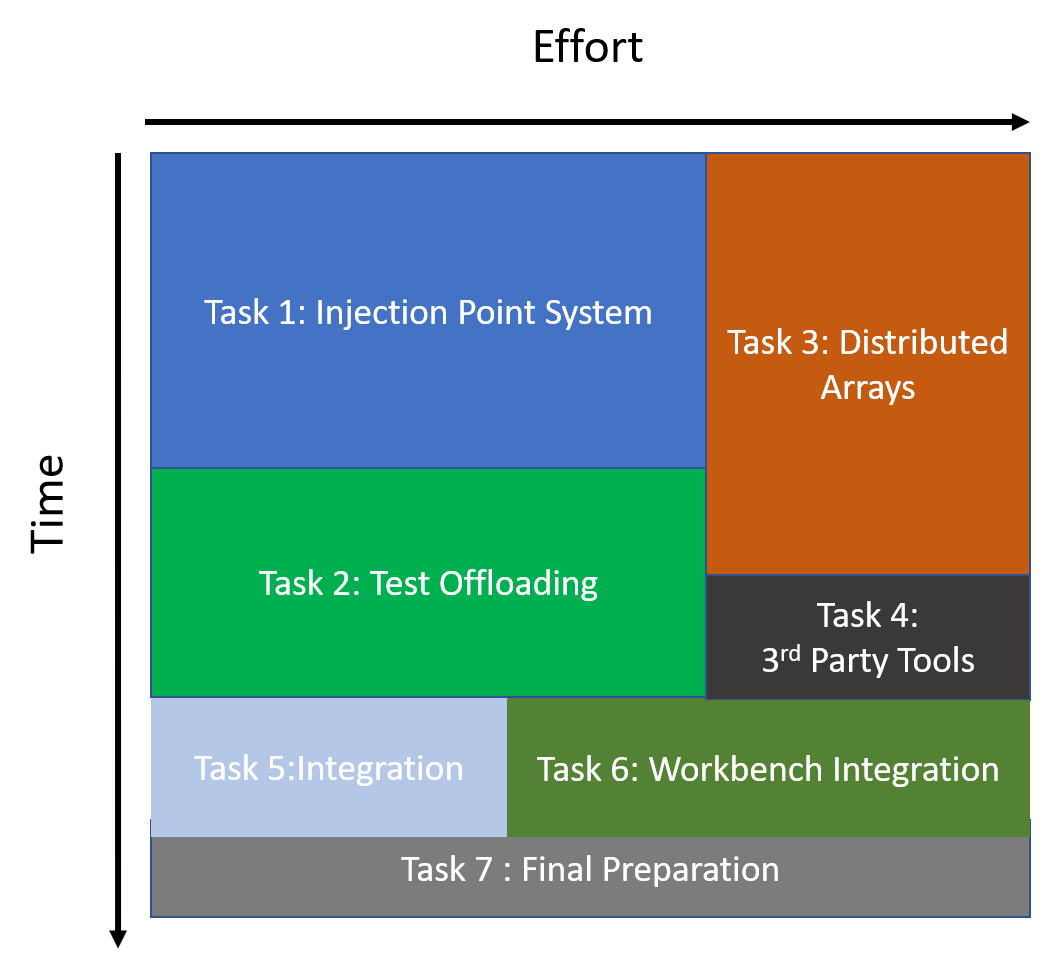
\includegraphics[width=1.0\linewidth]{./narrative/figures/tasks.pdf}
\end{center}
\caption{Overview of task dependencies and timeline.}
\label{fig:tasks}
\end{wrapfigure}

RNET would like to present the project ideas and research plan to the
DOE Program Manager and other interested scientists. The meeting will
be used to discuss features, and identify the specific NEAMS applications and computer
resources that will benefit from this project.  This meeting will be
scheduled soon after the Phase II contract is awarded. The meeting can
be hosted at RNET, a DOE site suggested by the Program Manager or via
a teleconference.

RNET will submit all reports as required by the contract (e.g., annual reports, 
a continuation report, summary reports, and a final report) to the DOE program 
manager and other interested DOE scientists.

The research and development topics described in Section~\ref{sec:workplan} 
will be addressed by the tasks described in the remainder of this section. Most 
tasks require active collaboration between RNET and its collaborators. 
Figure~\ref{fig:tasks} summarizes at a high level the dependencies among tasks  and
approximate anticipated task durations. The duration of the Phase II 
project is 104 weeks. Specific details are included in the description of each 
task.


\newcounter{taskCount}
\setcounter{taskCount}{0}

\refstepcounter{taskCount}\label{task:2.5}
\subsubsection{Task \ref{task:2.5}: Hardening of the Phase I VnV Injection Point System. }

In this task, the project team will develop an efficient, intuitive and type-safe injection point system for specifying testing points in, and across, advanced numerical software packages. Building on top of the Phase I prototype, this work will look to implement the injection point system in a way that allows for in-situ variable inspection in a robust and consistent way. The two main that need to be addressed are (1) the distinct lack of a robust reflection API in C++ makes defining functions that support generic arguments of unknown classes in a type safe way difficult, (2) the overhead associated with \VV injection points in cases where no testing is requested and (3) the difficulties in ensuring tests do not modify the variables in any way. Implementing this will require looking into the possibilities of implementing a LLVM compiler option for run-time removal of unused injection points, and/or the development of binary rewriting tools and the integration of parallel relative debugging techniques for detecting un-authorized and/or unintended changes is the run-time variables. 

\rnetprop{RNET will work on the implementation for this task and ORNL will provide inputs and guidance.}


\refstepcounter{taskCount}\label{task:3}
\subsubsection{Task \ref{task:3}: Develop methods for offloading tests to external processes. }
Performing a large number of \VV tests in a distributed environment will be expensive, both computationally and due to the data movement required to deal with the domain decomposition employed by the application. In this task, the project team will investigate the development of a mechanism for the evaluation of \VV tests that is lightweight and minimizes resource consumption. The initial approach to this will be to determine the requirements for efficient \VV test execution, and assess the capabilities provided by frameworks such as MRNet, SNOflake, ADIOS, etc. to determine if they can meet these requirements. Depending on the results of this assessment, work will be undertaken to create a library that can be integrated with the \VV framework. This library will be based on either one of these frameworks or using a custom solution. The project team will also determine the feasibility of integrating the Parallel Tools Platform (PTP) as a mechanism for minimizing \VV runtime through job parallelism. If appropriate, the team will extending PTP to fit this purpose.   

\rnetprop{RNET will work on the implementation for this task and ORNL will provide inputs and guidance.}

\refstepcounter{taskCount}\label{task:23}
\subsubsection{Task \ref{task:23}: Development of efficient statistical \VV tools with a focus of performance in large scale distributed settings.}

In this task, the team will perform R\&D work to determine and implement efficient statistical based \VV tools that can be applied in distributed settings. Consider that case of comparing the simulated solution to some known experimental results. In a distributed setting, the user must either distribute the experimental data across the nodes based on some known description of the data decomposition (difficult in a general setting), or gather to solution to some root node (expensive, and in many cases impossible. In this task, the project team will look into efficient mechanisms for inferring, detecting, and or describing the data decomposition such that this style of tests can be completed in an efficient manner. 

\rnetprop{RNET will be responsible for this task. ORNL will provide guidance on 
developing the framework for ORNL CADES.}

\refstepcounter{taskCount}\label{task:22}
\subsubsection{Task \ref{task:22}: Development of Generic tools for Mesh refinement, Uncertainty quantification and Sensitivity Analysis.}
In this task, RNET will implement generic \VV tools for mesh refinement, uncertainty quantification and sensitivity analysis. In the case of mesh refinement, the approach taken will be to create a generic interface for interacting with the automatic mesh refinement functionality that already exists in finite element libraries like LibMesh and Fenics. The overall goal is to create a generic VnV test that can be attached to the main function of the executable such that it automates the process of running mesh refinement and mesh convergence studies. In the case of UQ and SA, the project team will develop an interface for specifying the tools available in DAKOTA as VnV tests. 

\rnetprop{RNET will be responsible for this task. ORNL will provide guidance on 
developing the framework for ORNL CADES.}


\refstepcounter{taskCount}\label{task:4}
\subsubsection{Task \ref{task:4}: Extension of the VnV report generation system}
In this task, the project team will complete the development of the VnV report generation system. he primary goal of this task will be
to provide support for generating VnV reports that conform to the specification outlined in the DoD VV report templates.  The task will also include  a full implementation 
of the VnV markdown extension to support a wide variety of data visualization components, the development of the interfaces required for displaying unit and regression testing
reports, and the software indirections required for assimilating multiple VnV reports into a single document that can be used in the \VV of an entire simulation package. 

\rnetprop{RNET will work on the implementation for this task}

\refstepcounter{taskCount}\label{task:1}
\subsubsection{Task \ref{task:1}: Integration into real applications, including the NEAMS Tools}
\rnetprop{
  In this task, the program team will integrate the VnV framework into a variety of real applications. Initially, this 
  testing will be completed in tools used heavily in the NEAMS toolkit; MOOSE, libMesh and PETSc, but other third party 
  applications will also be investigated. To ensure seamless integration with the MOOSE tools, the project team will reimplement
  the XML based configuration file using the MOOSE input file format. This will allow for the configuration of the VnV tests in 
  a MOOSE application directly from the input file.
  
  The goal of this task will be to generate informative, production quality VnV 
  reports for a number of examples available in the MOOSE testing suite. Doing so allows us
  to test every facet of the proposed framework, while also acting the first demonstration of the
  value provided by the framework. These results of these tests will be hosted on the RNET website 
  as they become available. 
 

}

\rnetprop{
RNET will be responsible for this task and ORNL will provide guidance on 
various technical implementations and details.
}
\refstepcounter{taskCount}\label{task:11}
\subsubsection{Task \ref{task:11}: Development of an interface for the NEAMS workbench}
\rnetprop{
  In this task, the project team will integrate the toolkit directly into the NEAMS workbench. This will be
  a two stage process. First, the project team will implement the required interface files for enabling 
  the context aware auto-complete features available in the NEAMS workbench for the MOOSE based configuration
  file specification developed in the previous section. MOOSE based input files are already largely supported in
  the workbench; however, there will likely be some issues with determining which tests are applicable at which 
  injection points. Second will be developing an interface for customizing and viewing the final VV report. As part of the Phase I
  effort, the project team demonstrated viewing the final \VV report in a QT WebView component. The workbench is also but on to
  off QT, hence we do not expect to many difficulties on that front. Instead the key objective will be to develop the mechanisms for
  displaying customizations made the the final report in real-time within the NEAMS workbench. 
}
\rnetprop{ RNET will be responsible for this task }


\subsection{Facilities/Equipment}
\subsubsection{RNET Facilities}
RNET has the necessary office equipment to manage an SBIR/STTR contract
including networks, workstations, and accounting software. In
addition, RNET has the tools (software and hardware) to evaluate and
develop the technologies proposed here.  

RNET currently has 9 development computers and a 10-node development cluster 
that can be used for development and testing in this effort. Each cluster node 
has two quad-core or hexa-core XEON CPUs, 24-32GB of DRAM, 500+GB of local 
disk. 
Two data networks are available, a COTS 1 Gbps Ethernet network and a 10 Gbps 
Ethernet network. The Linux development nodes and the RNET cluster have the 
necessary Linux/GNU toolchains and development environments including; GNU 
tool chain, Microsoft .Net Framework, and Java Standard Edition.

\subsubsection{ORNL Facilities}
%\rnetcomment{Jay to verify, can we state these resources can be used on this project?}
The Oak Ridge National Laboratory (ORNL) hosts three petascale computing 
facilities: the Oak Ridge Leadership Computing 
Facility (OLCF), managed for DOE; the National Institute for Computational 
Sciences (NICS) computing facility operated 
for the National Science Foundation (NSF); and the National Climate-Computing 
Research Center (NCRC), formed as 
collaboration between ORNL and the National Oceanographic and Atmospheric 
Administration (NOAA) to explore a variety of 
research topics in climate sciences. Each of these facilities has a 
professional, experienced operational and engineering 
staff comprising groups in high-performance computing (HPC) operations, 
technology integration, user services, scientific 
computing, and application performance tools.

%\rnetcomment{Ram: Based on Jay's comments.}
ORNL also has the Compute and Data Environment for Science (CADES) which is a 
fully integrated infrastructure offering compute and data services for 
researchers lab-wide. We will work with appropriate program managers to apply 
for allocation requests as appropriate.


 The ORNL computer facility staff 
provides continuous operation of the centers 
and immediate problem resolution. On evenings and weekends, operators provide 
first-line problem resolution for users with 
additional user support and system administrators on-call for more difficult 
problems. ORNL also has state-of-the-art 
visualization facilities that can be used on site or accessed remotely. 
